\documentclass[12pt]{article}\usepackage[]{graphicx}\usepackage[]{color}
% maxwidth is the original width if it is less than linewidth
% otherwise use linewidth (to make sure the graphics do not exceed the margin)
\makeatletter
\def\maxwidth{ %
  \ifdim\Gin@nat@width>\linewidth
    \linewidth
  \else
    \Gin@nat@width
  \fi
}
\makeatother

\definecolor{fgcolor}{rgb}{0.345, 0.345, 0.345}
\newcommand{\hlnum}[1]{\textcolor[rgb]{0.686,0.059,0.569}{#1}}%
\newcommand{\hlstr}[1]{\textcolor[rgb]{0.192,0.494,0.8}{#1}}%
\newcommand{\hlcom}[1]{\textcolor[rgb]{0.678,0.584,0.686}{\textit{#1}}}%
\newcommand{\hlopt}[1]{\textcolor[rgb]{0,0,0}{#1}}%
\newcommand{\hlstd}[1]{\textcolor[rgb]{0.345,0.345,0.345}{#1}}%
\newcommand{\hlkwa}[1]{\textcolor[rgb]{0.161,0.373,0.58}{\textbf{#1}}}%
\newcommand{\hlkwb}[1]{\textcolor[rgb]{0.69,0.353,0.396}{#1}}%
\newcommand{\hlkwc}[1]{\textcolor[rgb]{0.333,0.667,0.333}{#1}}%
\newcommand{\hlkwd}[1]{\textcolor[rgb]{0.737,0.353,0.396}{\textbf{#1}}}%
\let\hlipl\hlkwb

\usepackage{framed}
\makeatletter
\newenvironment{kframe}{%
 \def\at@end@of@kframe{}%
 \ifinner\ifhmode%
  \def\at@end@of@kframe{\end{minipage}}%
  \begin{minipage}{\columnwidth}%
 \fi\fi%
 \def\FrameCommand##1{\hskip\@totalleftmargin \hskip-\fboxsep
 \colorbox{shadecolor}{##1}\hskip-\fboxsep
     % There is no \\@totalrightmargin, so:
     \hskip-\linewidth \hskip-\@totalleftmargin \hskip\columnwidth}%
 \MakeFramed {\advance\hsize-\width
   \@totalleftmargin\z@ \linewidth\hsize
   \@setminipage}}%
 {\par\unskip\endMakeFramed%
 \at@end@of@kframe}
\makeatother

\definecolor{shadecolor}{rgb}{.97, .97, .97}
\definecolor{messagecolor}{rgb}{0, 0, 0}
\definecolor{warningcolor}{rgb}{1, 0, 1}
\definecolor{errorcolor}{rgb}{1, 0, 0}
\newenvironment{knitrout}{}{} % an empty environment to be redefined in TeX

\usepackage{alltt}
\usepackage[utf8]{inputenc}
\usepackage[german]{babel}
\usepackage{apacite}
\usepackage{graphicx}
\usepackage{amsmath}
\usepackage{xcolor}
\usepackage{a4wide}
\usepackage[nottoc, numbib]{tocbibind}
\usepackage{natbib} 
\usepackage{booktabs}
\usepackage{longtable}
\usepackage{array}
\usepackage{multirow}
\usepackage{wrapfig}
\usepackage{float}
\usepackage{colortbl}
\usepackage{pdflscape}
\usepackage{tabu}
\usepackage{threeparttable}
\usepackage{threeparttablex}
\usepackage[normalem]{ulem}
\usepackage{makecell}
\usepackage{siunitx}

\renewcommand{\baselinestretch}{1.5}
\numberwithin{equation}{section}



\title{Analyse von hierarchischen Daten in R \\ mittels Multilevel Analyse}

\author{Masterarbeit von \\ Noah Bosshart \\ Mat-Nr.: 13-747-141 \\ \\ \\ Betreut durch \\ Prof. Dr. Carolin Strobl}
\IfFileExists{upquote.sty}{\usepackage{upquote}}{}
\begin{document}


\begin{figure}[t]
  \centering
  
\includegraphics[width = 8cm]{uzh_logo}
\end{figure}

\maketitle

\newpage
\tableofcontents

\newpage
\listoffigures

\newpage
\listoftables

\newpage
\section{Abstract}

\newpage

\section{Einleitung}
Hierarchische Daten treten häufig in den Sozialwissenschaften auf, unter anderem auch in der Psychologie \citep{SnijdersTomA.B2012Ma:a}. Von hierarchischen Daten wird gesprochen, wenn beispielsweise Daten von Schulkindern innerhalb verschiedener Schulklassen oder von Mitarbeitern aus mehreren Teams erhoben werden. Aber auch Daten aus Langzeitstudien werden als gruppiert bezeichnet, da mehrere Messzeitpunkte innerhalb einer Person gruppiert sind. Hierarchische Daten werden in Levels unterteilt, wobei Daten aus der niedrigsten Stufe als Level-1 Einheiten bezeichnet werden \citep{SnijdersTomA.B2012Ma:a}. Ein Beispiel für Level-1 Einheiten sind Schulkinder. Diese Schulkinder befinden sich wiederum in Klassen, die in der Hierarchiestufe höher sind und folglich als Level-2 Einheiten bezeichnet werden. Würde man nun in einer Studie nicht nur Schulkinder in Schulklassen, sondern auch  die Schulen selbst berücksichtigen, würden die Schulen als Level-3 Einheit bezeichnet werden. Die Anzahl der Levels könnte man theoretisch beliebig hoch wählen, solange es das Studiendesign erlaubt und es aus der Perspektive der Forschungsfrage sinnvoll ist. Der Einfachheit halber beschränken wir uns im Laufe dieser Arbeit aber auf hierarchische Daten mit zwei Levels. In Tabelle \ref{tab:beispiele_levels} werden einige Beispiele für Level-1 und Level-2 Einheiten aufgeführt. 

\begin{table}[h!]
\centering
\caption{Beispiele für Level-1 und Level-2 Einheiten}
\vspace{5mm}
\begin{tabular}{ll}
\toprule
Level-1 				& Level-2 	\\
\midrule
Schulkinder 			& Klasse 	\\
Studierende 			& Studienrichtungen \\
Kinder 					& Familien 	\\
Familien 				& Nachbarschaften \\
Mitarbeiter 			& Teams \\
Teams					& Unternehmen \\
Patienten 				& Therapeuten \\
Therapeuten 			& Kliniken \\
Mehrere Messzeitpunkte 	& Person \\
\bottomrule
\end{tabular}

\label{tab:beispiele_levels}
\end{table}

Dabei ist zu beachten, dass sich das Level der selben Einheit je nach Untersuchungsgegenstand ändern kann. Wie man in der Tabelle \ref{tab:beispiele_levels} erkennen kann, sind Familien einmal als Level-1 und einmal als Level-2 Einheit aufgeführt. Daher ist es wichtig die Level Bezeichnung nicht als starr zu betrachtet. Vielmehr sollte man sich grundsätzlich an den niedrigsten Einheiten im Datensatz orientieren. Diesen Einheiten wird dann das Level-1 zugeschrieben.

In der Forschung ist es aus Kostengründen oder aus Gründen des Studiendesigns oft nicht möglich, solche gruppierte Datenstrukturen zu vermeiden \citep{SnijdersTomA.B2012Ma:a, woltman2012introduction}. Als eine von vielen Ursachen, die zur Entstehung solcher Datenstrukturen führt, nennen Snijders und Bosker \citeyearpar{SnijdersTomA.B2012Ma:a} \textit{multistage sampling}. Unter \textit{multistage sampling} versteht man, dass die Forschenden in der Datenerhebung auf in der Population vorhandene Gruppen zugreifen. Beispielsweise ist es Kostengünstiger zufällig 100 Schulkassen und von diesen Schulklassen wieder jeweils 10 Kinder auszuwählen als von 1000 Schulklassen jeweils nur einen Schulkind auszuwählen. Da man sonst in 1000 verschiedenen Schulklassen eine Studie durchführen müsste, um die gleiche Stichprobengrösse zu erreichen. Dieses Auswahlverfahren führt dazu, dass die erhobenen Daten nicht mehr voneinander unabhängig sind. Werden nun aus jeder Schulklasse 10 Schulkinder für eine Studie ausgewählt, ist es sehr wahrscheinlich, dass Schulkinder aus der selben Klasse zueinander ähnlichere Leistungen erzielen werden. Dieser Zusammenhang kann auf unterschiedliche Ursache zurückzuführen sein. Beispielsweise könnte die didaktischen Fähigkeiten der Lehrpersonen oder die Lichtverhältnisse im Klassenzimmer einen Einfluss auf die Leistungen der Kinder aus der selben Klasse haben. Das heisst, dass Einflussfaktoren aus unterschiedlichen Levels sich gegenseitig beeinflussen können. 

Nach Snijders und Bosker \citeyearpar{SnijdersTomA.B2012Ma:a} gibt es unterschiedliche Formen, wie diese Einheiten zueinander in Beziehung stehen können. Ein Beispiel für einen Zusammenhang auf Level-1 wäre, dass die Lernmotivation eines Schulkindes sich auf seine Schulische Leistung auswirkt. Aber auch Level-2 Einheiten können sich gegenseitig beeinflussen. Das Klima der Schulklasse könnte sich beispielsweise auf das Stressempfinden der Lehrperson auswirken. Hier wird von einem Zusammenhang innerhalb des Levels gesprochen, weil die unabhängige Variable (z.B. Lernmotivation, Klima der Schulklasse) auf dem gleichen Level wie die abhängige Variable (z.B. schulische Leistung, Stressempfinden) ist. Häufig ist es allerdings der Fall, dass es levelübergreifende Zusammenhänge zwischen den Einheiten gibt. So können beispielsweise die didaktischen Fähigkeiten einer Lehrperson (Level-2) und die Lernmotivation der Schulkinder (Level-1) die individuelle Leistung (Level-1) beeinflussen. Dieser Zusammenhang muss nicht zwingend direkt sein. Es kann auch vorkommen, dass die didaktischen Fähigkeiten den Zusammenhang zwischen Lernmotivation und individueller Leistung moderiert. In diesem Fall wird gemäss Snijders und Bosker \citeyearpar{SnijdersTomA.B2012Ma:a} von einer \textit{cross-level interaction} gesprochen.

Werden diese Abhängigkeiten in der Analyse nicht berücksichtigt, kann dies zu einer erhöhten Fehler Typ-1 Rate führen \citep{dorman2008effect, mcneish2014analyzing}. Das heisst, dass Forschende vermehrt zu Fehlschlüssen bezüglich des Einflusses ihrer Abhängigen Variablen gelangen und irrtümlich annehmen, einen Effekt eines Verfahren gefunden zu haben, obwohl es diesen Effekt gar nicht gibt. Das Vorhandensein von hierarchischen Daten ist allerdings kein unlösbares Problem. Mit Analyseansätzen, die diese hierarchische Struktur der Daten berücksichtigen, lassen sich solche erhöhten Fehler Typ-1 Raten vermeiden. Einer dieser Ansätze ist die Multilevel Analyse, die im Fokus dieser Arbeit steht.

Diese Arbeit ist in drei Teile unterteilt. Im ersten Teil wird das Konzept und die Theorie der Multilevel Analyse behandelt. Dabei wird kurz auf die verschiedenen Methoden eingegangen, wie man Daten auf ihre hierarchische Struktur überprüfen kann. Anschliessend wird das zugrundeliegende statistische Modell der Multlilevel Analyse vorgestellt und wie genau solche Modelle aufgebaut sind. Darauf folgend wird die Anwendung dieser Methoden in der Statistikumgebung R besprochen \citep{R}. Im zweiten Abschnitt dieser Arbeit wird eine Simulationsstudie durchgeführt, deren Ziel es ist, bereits vorhandene Ergebnisse in der Literatur zu replizieren und da Daseinsberechtigung von Mulitlevel Analyse von hierarchischen Daten zu festigen. Im dritten und letzten Abschnitt wird eine eigens programmierte Shiny Web-App vorgestellt \citep{shiny}, die zum einen das Konzept der Multilevel Analyse visualisiert und dem Nutzer die Möglichkeit gibt, selbst die Simulationsstudie aus dem zweiten Abschnitt durchzuführen. 

\section{Konzept und Anwendung von Multilevel Analyse}
Wie in der Einleitung erläutert wurde, gibt es viele Situationen in denen hierarchische Daten vorhanden sind und wenn diese Strukturen nicht berücksichtigt werden, kann man zu Fehlschlüssen gelangen. In diesem Abschnitt wird nun etwas genauer auf das Konzept und die dahintersteckende Theorie der Multilevel Analyse eingegangen. 
Dazu wird zuerst ein simulierter Beispieldatensatz vorgestellt. Anhand dieses Beispiels werden Probleme aufgezeigt, die entstehen, wenn man einfache lineare Modelle verwendet und anschliessend wird das hierarchische lineare Modell (HLM) eingeführt. Das HLM ist das zugrundeliegendes statistisches Modell der Multilevel Analyse und gilt als eine Erweiterung des einfachen linearen Modells \cite{SnijdersTomA.B2012Ma:a}. Dabei werden bei HLMs in \textit{random intercept} und \textit{random intercept and slope} Modelle unterschieden. und erläutert wie die beiden Faktoren Achsenabschnitt (engl. \textit{intercept}) und Steigung (engl. \textit{slope}) zusammenhängen. Nachdem die verschiedenen Formen von HLMs besprochen worden sind, wird in einem etwas praktischeren Teil die Anwendung von Multilevel Analyse in R anhand von Beispielen etwas näher gebracht.

\subsection{Beispiel zur Theorie}
In den folgenden Abschnitten wird die Theorie zur Analyse von hierarchischen Daten anhand eines Beispieldatensatzes erläutert. Bei dem Beispiel handelt es sich um insgesamt 150 Schulkindern aus 5 Schulklassen, die eine Mathematikprüfung geschrieben haben. Neben der erreichten Punktzahl wurde für jedes Kind zufällig ein Geschlecht, die Anzahl an gelösten Übungen, einen Wert für sozioökonomische Status und einen Intelligenzquotienten simuliert. Auf Stufe der Klasse wurden ausserdem noch die Anzahl Fenster im Klassenzimmer simuliert. Da dieser Datensatz selbst generiert wurde und aus keiner Studie entstammt, sollten Ergebnisse, die aus diesen Berechnungen entstehen nicht weiter interpretiert werden. Eine genaue Erläuterung wie dieser Datensatz generiert wurde, ist im Abschnitt über die Generierung von hierarchischen Daten zu finden. In Tabelle \ref{tab:beispiel_theorie} sind zur Veranschaulichung die Daten von 10 Schulkindern aufgeführt.

\begin{table}[ht]
\centering
\caption{Ausschnitt des simulierten Datensatzes} 
\vspace{5mm}
\begin{tabular}{cccccccc}
  \toprule
 Schulkind Nr. & Klasse & Übungen & Punktzahl & Geschlecht & Anz. Fenster & SES & IQ \\ 
  \midrule
101 & 4 & 17 & 21 & m & 3 & 16 & 104 \\ 
  75 & 3 & 7 & 29 & m & 8 & 27 & 112 \\ 
  126 & 5 & 23 & 26 & w & 4 & 14 & 110 \\ 
  14 & 1 & 10 & 29 & m & 4 & 21 & 84 \\ 
  137 & 5 & 16 & 18 & w & 4 & 17 & 109 \\ 
  100 & 4 & 7 & 16 & w & 3 & 20 & 98 \\ 
  78 & 3 & 28 & 44 & w & 8 & 23 & 105 \\ 
  121 & 5 & 25 & 33 & w & 4 & 21 & 99 \\ 
  16 & 1 & 7 & 24 & w & 4 & 30 & 77 \\ 
  116 & 4 & 14 & 29 & m & 3 & 19 & 90 \\ 
   \bottomrule
\end{tabular}
\label{tab:beispiel_theorie}
\end{table}

Betrachtet man die Ausprägung einzelner Variablen des Datensatzes, kann man erkennen, dass gewisse Variablen sich nicht zwischen den Schulkindern verändern. Wenn sich Variablen über einzelne Beobachtungen hinweg nicht verändern, kann das ein Hinweis dafür sein, dass es sich um hierarchische Daten handelt. Unser Datensatz hat in der Tat ein hierarchische Struktur mit zwei Levels. Zu den Level-1 Variablen gehören alle Variablen die sich auf der Stufe der tiefsten Einheit (Schulkinder) befinden. Dazu zählen die Anzahl gelösten Übungen, die erreichte Punktzahl, das Geschlecht, der sozioökonomische Status und der IQ. Die beiden anderen Variablen Klasse und die Anzahl Fenster im Klassenzimmer gehören zu Level-2.

\subsection{Lineare Modelle}
Bevor wir uns mit den hierarchischen linearen Modellen beschäftigen, werden hier noch einmal kurz die Grundlagen der linearen Regression erläutert. Gemäss Gelman und Hill \citeyearpar{andrew_data} ist die lineare Regression eine Methode, die Veränderungen von Durchschnittswerten einer abhängigen Variablen durch eine lineare Funktion von Prädiktoren beschreibt. In etwas einfacheren Worten ausgedrückt, versucht die lineare Regression durch die Kombination von unabhängigen Variablen die mittlere Ausprägung einer abhängigen Variable zu beschreiben. Ein lineares Regressionsmodell kann wie folgt formuliert werden:
\begin{equation}
y_{i} = \beta_{0} + \beta_{1}X_{i1} + \dots + \beta_{ik}X_{ik} + \epsilon_{i}, \text{ für } i = 1, \dots, n \text{ und } \epsilon_{i} \sim \mathcal{N}(0,\sigma^{2})
\end{equation}

Dabei ist $y_{i}$ die abhängige Variable von der Person $i$. In unserem Beispiel wäre das die erreichte Punktzahl des Schulkindes $i$. $\beta_0$ beschreibt den Achsenabschnittes (\textit{intercept}) und ist die durchschnittlich erreichte Punktzahl in der Mathematikprüfung, wenn keine weitere Prädiktoren berücksichtigt werden. Die weiteren Regressionskoeffizienten $\beta_{1}$ bis $\beta_{k}$ beschreiben für jede unabhängige Variable $X_{i1}$ bis $X_{ik}$ wie stark $y_{i}$ des $i$-ten Schulkindes bei einer Zunahme um eine Einheit ansteigt. Die Regressionskoeffizienten $\beta_{1}$ bis $\beta_{k}$ beschreiben also die Steigung (\textit{slope}). Möchten wir in unserem Beispiel die erreichte Punktzahl durch die Anzahl gelöster Übungsaufgaben beschreiben, wäre $X_{i1}$ die Anzahl gelöster Übungsaufgaben des $i$-ten Schulkindes und der dazugehörige Regressionskoeffizient $\beta_{1}$ gibt die Zunahme der Punktzahl in der Mathematikprüfung an. Der letzte Koeffizient des Regressionsmodells ist $\epsilon_{i}$ und wird als zufälliger Fehler oder Residuum bezeichnet. Das Residuum ist die normal verteilte zufällige Abweichung jedes $i$-ten Schulkindes, mit einem Erwartungswert von 0 und Varianz von $\sigma^{2}$. Das bedeutet, dass es zwischen den Kindern zufällige Unterschiede in ihrer Prüfungsleistung gibt, die nicht durch das Regressionsmodell erfasst werden. Diese Unterschiede sind im Mittel aber 0. 

\subsubsection{Aggregation}

Möchten man nun den Einfluss von Übungsaufgaben auf die erreichte Punktzahl in der Mathematikprüfung untersuchen, gibt es zwei Möglichkeiten, wie man mit dem linearen Regressionsmodell diese Frage überprüfen kann. Bei der ersten Möglichkeit würde man für jede Klasse die Mittelwerte für die Prüfungsleistung und die Anzahl gelöster Übungsaufgaben berechnen und anhand dieser Mittelwerte die Forschungsfrage untersuchen. Diese Methode wird in der Literatur als Aggregation bezeichnet \citep{SnijdersTomA.B2012Ma:a, woltman2012introduction}. In Tabelle \ref{tab:aggregation} wurde für jede der fünf Schulklassen die Durchschnittswerte berechnet.

\begin{table}[ht]
\centering
\caption{Durchschnittliche Anzahl gelöster Übungsaufgaben und erreichte Punktzahl}
\vspace{5mm}
\begin{tabular}{ccc}
  \hline
Klasse & Übungen & Punktzahl \\ 
  \hline
1 & 13.1 & 21.5 \\ 
2 & 12.8 & 29.3 \\ 
3 & 13.5 & 30.7 \\ 
4 & 15.7 & 25.6 \\ 
5 & 17.5 & 24.7 \\ 
   \hline
\end{tabular}
\label{tab:aggregation}
\end{table}

Wird nun anhand dieser aggregierter Werte überprüft, wie genau die erreichte Punktzahl eines Schulkindes mit der Anzahl an gelösten Übungsaufgaben zusammenhängt, entstehen mehrere Probleme, die zu Verzerrungen und Fehlschlüssen führen können. Zum einen verändert sich die Forschungsfrage, da sich durch die Aggregation der Daten der Fokus von der Level-1 Ebene auf die Level-2 Ebene verschiebt \citep{SnijdersTomA.B2012Ma:a, woltman2012introduction}. Die abhängige Variable ist nun nicht mehr die erreichte Punktzahl jedes einzelnen Schulkindes, sondern die durchschnittlich erreichte Punktzahl einer Schulklasse. Ein weiteres Problem ist der Verlust von Variabilität, die durch individuelle Unterschiede zwischen den Schulkindern entsteht \citep{raudenbush2002hierarchical}. Dieser Verlust an Variabilität beträgt nach Raudenbush und Bryk \citeyearpar{raudenbush2002hierarchical} 80-90\% und kann zu massiven Fehlschlüssen über den Zusammenhang der Variablen führen. Einer dieser Fehlschlüsse wird als ökologischer Fehlschluss bezeichnet \citep{SnijdersTomA.B2012Ma:a}. Ein ökologischer Fehlschluss entsteht, wenn man unzulässigerweise aufgrund von aggregierten Ausprägungen eines Merkmals auf die Ausprägung dieses Merkmals in Individuen schliesst \citep{robinson2009ecological}. 

Dieser ökologische Fehlschluss lässt sich relativ einfach an unserem Beispiel erklären. Betrachtet man die Regressionsgerade in Abbildung \ref{fig:aggregiert}, könnte man daraus schliessen, dass die Anzahl gelöster Übungsaufgaben in einem negativen Zusammenhang mit der erreichten Punktzahl in der Mathematikprüfung stehen. 

\begin{figure}[hb!]
\centering
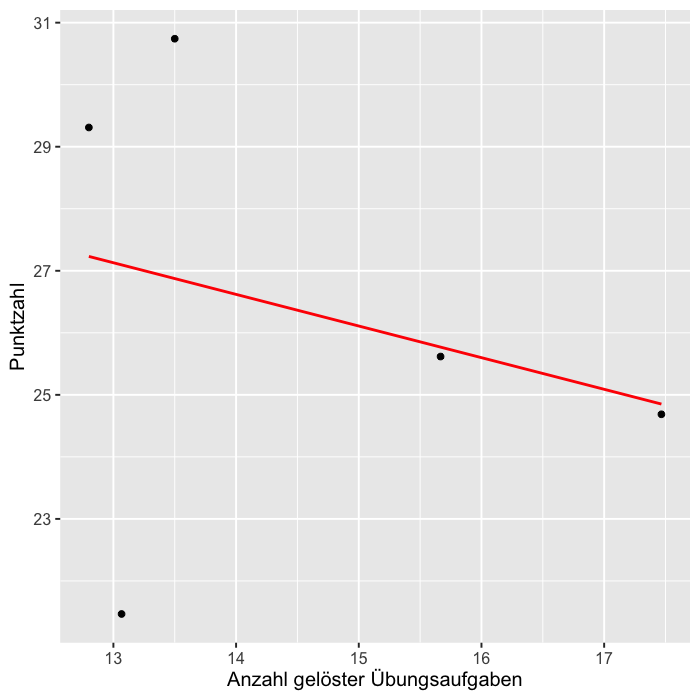
\includegraphics[width = 10cm, height = 10cm]{aggregation}
\caption{Zusammenhang zwischen der durchschnittlich gelösten Anzahl an Übungsaufgaben und der durschnittlich erreichten Punktzahl pro Klasse}
\label{fig:aggregiert}
\end{figure}

\subsubsection{Disaggregation}

\subsection{Hierarchische Linearen Modelle}
Hierarchische Lineare Modelle sind, wie bereits angedeutet eine Erweiterung von einfachen linearen Regressionsmodellen. 


\subsubsection{Intraklassen Korrelation}
Besprechen von ICC und Design Effekt (Vlg. Dazu Guide ML Analysis von J. Peugh 2009)
\subsubsection{\textit{Random Intercept} Modell}
\subsubsection{\textit{Random Intercept and Slope} Modell}

\subsection{Anwendung von Multilevel Analyse in R}
\subsubsection{R Pakete für die Multilevel Analyse}
Beschreibung von lme4 und grund warum in dieser Arbeit nur mit diesem Paket gearbeitet wird. (Buch und Studie von D. Bates)
\subsubsection{Aufbau eines Modells}
Die meisten Modelle erlauben nicht mehr als 2-3 Random Slopes und konvergieren nicht \citep{SnijdersTomA.B2012Ma:a}
\subsubsection{Interpretation des Outputs}

\subsubsection{Vergleich von Hierarchischen Linearen Modellen}
Modelle welche sich nur in fixen Effekten unterscheiden sollten mit ML und Modelle welche sich in zufälligen Effekten unterscheiden mit REML verglichen werden \cite{SnijdersTomA.B2012Ma:a}

Tests für feste Effekte Wald-Test \cite{SnijdersTomA.B2012Ma:a} Inkl. Dummy-Test

Deviance Tests ebenfalls verwendbar für feste Effekte. Bei Random Intercept an chi-square verteilung mit df = anz. veränderte variable teile (wichtig fixed effect müssen gleich bleiben, wenn mit REML, sonst ML)

Da Varianzen nicht negativ werden können, wird oft einseitig getestet. Konservativere Möglichkeit druch halbierung des testwertes ("Zweiseitiges Testen").


Deviance Tests für Random Slope etwas aufwändiger, df = m1 - m0 = p + 1 (anz. covarianzen p, von denen sich das m0 zu m1 unterscheiden + 1 varianz) Prüfwert wird für df = p und für df = p+1 in einer chi-quadrat verteilung bestimmt. danach mittelwert davon ergibt den eigentlichen prüfwert. 

Konfidenzintervall am besten durch profile likelihood (via lme4 Paket). Profile likelihood verhindert, dass Konfidenzintervalle den Wert 0 Unterschreiten, da Varianzen nicht negativ sein können. 

Wenn diese Methode nicht vorhanden ist können andere Methoden gewählt werden, die allerdings nicht so genau/reliabel sind.

Proportionale Reduktion der Varianz und Pseude R Squared (Zitation nötig!)

\section{Simulationsstudie zur Multilevel Analyse}
\subsection{Herleitung der Forschungsfrage}
Es gibt schon Tutorials etc. wie man HLM in der Forschung einsetzt. Dabei achten auf Kennwerte (ICC und DEFF). Studien haben gezeigt, dass Fehler Typ-1 Rate steigt wenn MLM anstatt HLM) Studien zitieren, Dorman, Neith, Etc. Es stellt sich aber auch die Frage, wie es genau mit Treatments aussieht (studie treatment zitieren) auch diese haben einen erhöhte Typ-1 Rate gefunden. Ziel: replikation der ergebnisse, dass Fehler typ-1 rate erhöht ist und in einen für psychologiestudenten relevanten kontext bringen um das Konzept der HLM den studierenden zu verkaufen. 
H1: betas werden genau geschätzt
H2: SE bei Effekt von 0 zu klein bei MLM -> folglich zu viele p-werte < 0.05
\subsection{Design der Simulationsstudie}
\subsubsection{Generierung von hierarchischen Daten}
\subsubsection{Manipulierte Faktoren}
\subsubsection{Konstante Faktoren}
\subsubsection{Untersuchte Faktoren}
\subsection{Ergebnisse der Simulationsstudie}

\section{Beschreibung und Anwendung der Shiny App}
\subsection{Was ist Shiny?}
\subsection{Ziel der Shiny App}
\subsection{Anwendung der Shiny App}

\section{Diskussion}
\newpage
\bibliography{literatur_masterarbeit}
\bibliographystyle{apacite}

\section{Anhang}
\appendix
\section{R Code}





\end{document}
